\documentclass[conference]{IEEEtran} 
\IEEEoverridecommandlockouts 

\usepackage{cite}
\usepackage{amsmath,amssymb,amsfonts}
\usepackage{graphicx}
\usepackage{textcomp}
\usepackage{xcolor}
\usepackage{booktabs}
\usepackage{url}
\usepackage{graphicx}
\usepackage{tikz}
\usetikzlibrary{arrows.meta,positioning}


\def\BibTeX{{\rm B\kern-.05em{\sc i\kern-.025em b}\kern-.08em
    T\kern-.1667em\lower.7ex\hbox{E}\kern-.125emX}}

\begin{document}

\title{Calibrated Supervised Learning for Housing Price Prediction: A Probabilistic Inference Approach}

\author{
\IEEEauthorblockN{Annabel Irani}
\IEEEauthorblockA{\textit{Department of Computer Science} \\
\textit{Western University}\\
London, Canada \\
airani9@uwo.ca}
\and
\IEEEauthorblockN{Christopher Betancur}
\IEEEauthorblockA{\textit{Department of Computer Science} \\
\textit{Western University}\\
London, Canada \\
cbetancu@uwo.ca}
\and
\IEEEauthorblockN{Xiaowei Feng}
\IEEEauthorblockA{\textit{Department of Computer Science} \\
\textit{Western University}\\
London, Canada \\
xfeng282@uwo.ca}
}

\maketitle

\begin{abstract}
This report explores how supervised learning can be combined with uncertainty-aware postprocessing to predict housing prices more reliably. Using the California Housing Prices dataset from Kaggle~\cite{californiaKaggle}, we first build a transparent baseline with linear regression on standardized features. We then train a feedforward neural network (ReLU, Adam optimizer~\cite{kingma2015adam}) to model nonlinear relationships that the linear model cannot capture. To quantify how confident the system is in its point forecasts, we apply conformal prediction~\cite{angelopoulos2021} to produce calibrated prediction intervals that require minimal distributional assumptions. All models are implemented in Python using the Scikit-learn ecosystem~\cite{pedregosa2011}. The project illustrates a central CS3346 idea: accurate predictors are useful, but predictors that can also report well-calibrated uncertainty are more actionable.
\end{abstract}

\begin{IEEEkeywords}
supervised learning, regression, probabilistic inference, calibration, uncertainty quantification
\end{IEEEkeywords}

% -------------------------------------------------------------
\section{Introduction}\label{sec:intro}
Artificial Intelligence (AI) systems learn patterns from data to approximate complex functions and make predictions about real-world quantities. 
Within the CS3346: \emph{Artificial Intelligence} framework, this project falls under the module \emph{Intelligence from Data}, 
which focuses on how machines learn from examples, generalize to unseen cases, and reason under uncertainty. 
The project demonstrates these ideas through a practical supervised learning task: predicting housing prices using real-world socioeconomic data.

The California Housing dataset~\cite{californiaKaggle} is a widely used benchmark for regression analysis. 
It contains socioeconomic and geographic attributes for California districts, including variables such as 
median income, housing median age, total rooms, total bedrooms, population, households, and geographic 
coordinates (latitude and longitude). Predicting the median home value from these attributes illustrates key 
challenges in supervised learning, including bias–variance trade-offs, feature relevance, and model 
interpretability. Although the dataset is relatively compact, its real-world structure makes it useful for 
demonstrating foundational concepts in regression modeling.

To evaluate different modeling strategies, we employ both linear and nonlinear methods. 
Linear regression provides an interpretable baseline model for housing price prediction. 
For nonlinear modeling, we utilize neural networks to capture complex feature interactions that linear models cannot represent. 
These models are implemented using the Scikit-learn library~\cite{pedregosa2011}, which offers standardized APIs and reproducible workflows.

While point predictions are valuable, real-world decision-making often requires an understanding of uncertainty. 
Therefore, we extend the analysis with probabilistic techniques that estimate confidence around predictions. 
Specifically, conformal prediction~\cite{angelopoulos2021} is used to construct calibrated intervals that guarantee a desired coverage probability without assuming specific data distributions. 
This aligns with the \emph{probabilistic inference} component of CS3346, emphasizing that intelligent systems should not only predict but also measure their confidence.

Overall, this study aims to integrate core AI principles—learning from data, reasoning under uncertainty, and ensuring interpretability—within a compact yet meaningful application. 
The remainder of this paper is organized as follows: Section~\ref{sec:methodology} outlines the modeling methodology; Section~\ref{sec:implementation} describes implementation details; Section~\ref{sec:results} presents experimental results and discussion; and Section~\ref{sec:conclusion} concludes with key takeaways and future directions.

% -------------------------------------------------------------
\section{Methodology}\label{sec:methodology}

\subsection{Dataset}
We used the publicly available \emph{California Housing Prices} dataset from Kaggle~\cite{californiaKaggle}. 
Each instance corresponds to a California district and includes socioeconomic and geographic attributes such as 
median income, housing median age, total rooms, total bedrooms, population, households, and geographic location 
(latitude and longitude). The target variable is \emph{median\_house\_value}, which we aim to predict. After loading 
the dataset, we removed rows with missing or clearly invalid entries to ensure that the downstream models were 
trained on clean data. Features (inputs) and the target (output) were then separated into \(\mathbf{X}\) and \(y\), 
respectively.

\subsection{Feature Standardization}
Most input attributes are continuous and measured on different scales (e.g., income vs.\ longitude). To prevent features with large numeric ranges from dominating the learning process, we standardized all continuous features using the z-score transformation:
\begin{equation}
    x^{\prime} = \frac{x - \mu}{\sigma},
\end{equation}
where \(\mu\) and \(\sigma\) are the sample mean and standard deviation computed from the training data. The same statistics were applied to the validation and test splits to avoid data leakage. Standardization is especially important for gradient-based models, as it improves numerical stability and ensures comparable learning rates across features.

\subsection{Train--Validation--Test Split}
To assess generalization fairly, we randomly partitioned the dataset into three disjoint subsets: \(70\%\) for training, \(15\%\) for validation, and \(15\%\) for testing. A fixed random seed was used so that the split is reproducible. The training set was used to fit model parameters, while the validation set monitored performance and guided hyperparameter selection (e.g., number of hidden layers, neurons, learning rate). The test set was held out for final reporting to provide an unbiased estimate of model performance.

\subsection{Baseline: Linear Regression}
As a first model, we trained an ordinary least squares linear regressor on the standardized features to predict \emph{median\_house\_value}. This baseline captures only linear relationships between the housing attributes and the target, and it serves as a reference point for determining whether more expressive models provide meaningful improvements.

\subsection{Neural Network Regressor}
Our main model was a feedforward neural network for regression. The network took the standardized feature vector as input, passed it through one or more fully connected hidden layers with ReLU activations, and produced a single scalar output representing the predicted house value. The network was trained using mean squared error (MSE) loss and optimized with the Adam optimizer~\cite{kingma2015adam}. Training was conducted on the \(70\%\) training split, while the \(15\%\) validation split was used for early stopping and hyperparameter tuning. All models were implemented in Python using the Scikit-learn library~\cite{pedregosa2011}.

\subsection{Evaluation}
After training, we evaluated both the linear regression baseline and the neural network on the held-out \(15\%\) test set. We reported standard regression metrics such as mean squared error (MSE) and mean absolute error (MAE) to determine whether the nonlinear neural network provided a meaningful improvement over the linear baseline. These metrics allow us to compare not only overall accuracy but also robustness to large errors.

% -------------------------------------------------------------
\section{Implementation}

\subsection{Environment and Libraries}
All experiments were implemented in Python using open-source libraries. We used \texttt{pandas} and \texttt{NumPy} for data loading and manipulation, and the \texttt{scikit-learn} library~\cite{scikit-learn} for preprocessing, model training, and evaluation. Diagnostic plots were generated with \texttt{matplotlib}. A fixed random seed (\texttt{random\_state = 42}) was set wherever possible so that the train--validation--test split and the optimization procedure of the models could be reproduced across runs.

\subsection{Data Loading and Cleaning}
The California Housing Prices dataset was stored locally as a CSV file. We loaded it using \texttt{pandas.read\_csv}, inspected the columns, and removed rows with missing values. The target column \texttt{Median\_House\_Value} was extracted into a vector $y$, and the remaining columns (including \texttt{Median\_Income}, \texttt{Median\_Age}, \texttt{Tot\_Rooms}, \texttt{Tot\_Bedrooms}, \texttt{Population}, \texttt{Households}, \texttt{Latitude}, \texttt{Longitude}, and several distance features) were treated as the feature matrix $X$. Each row therefore corresponds to one census block group, and the task is to predict a real-valued house price.

\subsection{Preprocessing and Standardization}
Most input attributes are continuous and measured on different scales (e.g., median income versus longitude). To prevent features with large numeric ranges from dominating the learning process, we standardized all continuous features using the $z$-score transformation
\begin{equation}
    x' = \frac{x - \mu}{\sigma},
\end{equation}
where $\mu$ and $\sigma$ are the sample mean and standard deviation computed from the \emph{training} data. We used the \texttt{StandardScaler} class from \texttt{scikit-learn} to fit these statistics on the training split only, and then applied the same transformation to the validation and test splits to avoid data leakage. The standardized features were stored as NumPy arrays for efficient model training.

\subsection{Train--Validation--Test Split}
To assess generalization fairly, we randomly partitioned the dataset into three disjoint subsets: $70\%$ for training, $15\%$ for validation, and $15\%$ for testing. This was implemented by first calling \texttt{train\_test\_split} to separate $30\%$ of the data into a temporary set and then splitting that temporary set evenly into validation and test subsets. The training set was used to fit model parameters, the validation set was used for model selection and hyperparameter tuning, and the test set was held out for final evaluation only. The overall pipeline is summarized in Figure~\ref{fig:pipeline}.

\begin{figure}[t]
\centering
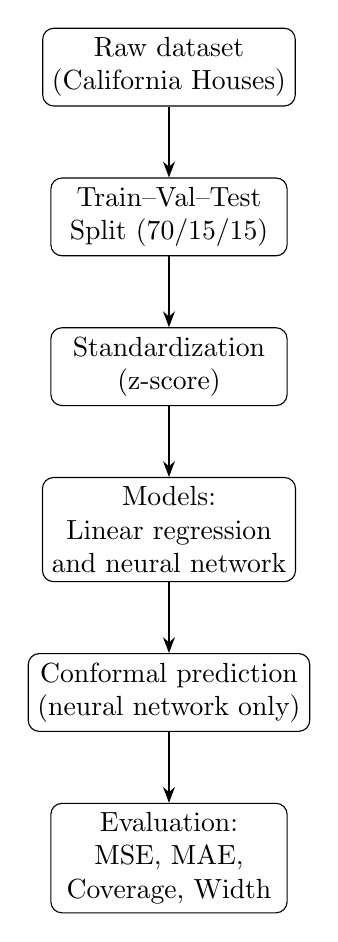
\begin{tikzpicture}[
  node distance=0.9cm,
  process/.style={
    rectangle,draw,rounded corners,
    minimum width=3.0cm,minimum height=0.8cm,
    align=center
  },
  arrow/.style={-{Stealth[length=2mm]},thick}
]

\node[process] (data) {Raw dataset\\(California Houses)};
\node[process, below=of data] (split) {Train--Val--Test\\Split (70/15/15)};
\node[process, below=of split] (std) {Standardization\\(z-score)};
\node[process, below=of std] (models) {Models:\\Linear regression\\and neural network};
\node[process, below=of models] (conf) {Conformal prediction\\(neural network only)};
\node[process, below=of conf] (eval) {Evaluation:\\MSE, MAE,\\Coverage, Width};

\draw[arrow] (data) -- (split);
\draw[arrow] (split) -- (std);
\draw[arrow] (std) -- (models);
\draw[arrow] (models) -- (conf);
\draw[arrow] (conf) -- (eval);

\end{tikzpicture}
\caption{Overall pipeline: raw data are split into training, validation, and test sets, standardized, and then passed to both a linear regression baseline and a neural network. The neural network output is further wrapped in a conformal prediction layer to obtain calibrated intervals. All models are evaluated on the held-out test set.}
\label{fig:pipeline}
\end{figure}

\subsection{Linear Regression Baseline}
As a transparent and interpretable baseline, we trained an ordinary least squares linear regressor using \texttt{LinearRegression} from \texttt{scikit-learn}. The model was fit on the standardized training features and then evaluated on the validation and test splits. For each split we computed the mean squared error (MSE)
\begin{equation}
    \text{MSE} = \frac{1}{n}\sum_{i=1}^{n}(y_i - \hat{y}_i)^2
\end{equation}
and the mean absolute error (MAE),
\begin{equation}
    \text{MAE} = \frac{1}{n}\sum_{i=1}^{n}\lvert y_i - \hat{y}_i \rvert,
\end{equation}
where $y_i$ and $\hat{y}_i$ denote the true and predicted house values for example $i$. These metrics provide an interpretable reference for absolute error levels and establish a baseline against which we can judge whether the neural network and conformal predictor provide meaningful improvements.

\subsection{Neural Network Regressor}
For nonlinear modeling, we used the \texttt{MLPRegressor} class from \texttt{scikit-learn} to implement a feedforward neural network. The network took the standardized feature vector as input, passed it through fully connected hidden layers with rectified linear unit (ReLU) activations, and produced a single scalar output representing the predicted house value. Training used mean squared error loss and the Adam optimizer~\cite{kingma2015adam}, which adaptively scales the learning rate for each parameter.

Rather than fixing the architecture a priori, we performed a small grid search over the number of hidden units and the learning rate. Concretely, we considered hidden layer configurations $(32)$, $(64)$, and $(64, 32)$ and learning rates $\{10^{-3}, 5\times10^{-4}\}$. For each configuration we trained an \texttt{MLPRegressor} with a maximum of $500$ iterations. The model was equipped with \emph{early stopping} using an internal validation fraction of the training data: if the internal validation loss did not improve for several epochs, training was halted automatically and the best weights so far were retained. After training each configuration, we evaluated its MSE on the explicit $15\%$ validation split and selected the model with the lowest validation MSE as our final neural network. The chosen architecture consisted of two hidden layers with 64 and 32 units respectively, as illustrated in Figure~\ref{fig:nn-architecture}.

\begin{figure}[t]
\centering
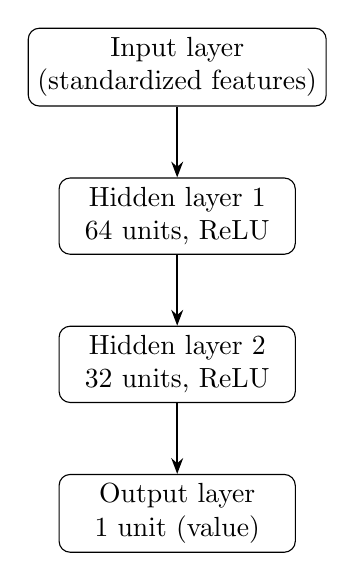
\begin{tikzpicture}[
  layer/.style={
    rectangle,draw,rounded corners,
    minimum width=3.0cm,minimum height=0.8cm,
    align=center
  },
  arrow/.style={-{Stealth[length=2mm]},thick}
]

\node[layer] (input) {Input layer\\(standardized features)};
\node[layer, below=0.9cm of input] (h1) {Hidden layer 1\\64 units, ReLU};
\node[layer, below=0.9cm of h1] (h2) {Hidden layer 2\\32 units, ReLU};
\node[layer, below=0.9cm of h2] (output) {Output layer\\1 unit (value)};

\draw[arrow] (input) -- (h1);
\draw[arrow] (h1) -- (h2);
\draw[arrow] (h2) -- (output);

\end{tikzpicture}
\caption{High-level architecture of the neural network used in our experiments. The final model has two hidden layers with 64 and 32 units respectively and ReLU activations.}
\label{fig:nn-architecture}
\end{figure}

\subsection{Uncertainty Estimation with Conformal Prediction}
To obtain calibrated prediction intervals around the neural network predictions, we implemented a split-conformal prediction procedure following Angelopoulos and Bates~\cite{angelopoulos2021}. After fitting the final neural network on the training data with the selected hyperparameters, we used the validation split as a calibration set. We computed the absolute residuals between predicted and true values on this set,
\begin{equation}
    r_i = \lvert y_i - \hat{y}_i \rvert,
\end{equation}
and took the $(1 - \alpha)$ quantile of this residual distribution (e.g., the $90$th percentile for a nominal $90\%$ interval). At test time, we formed symmetric prediction intervals by subtracting and adding this quantile to each point prediction,
\begin{equation}
    [\hat{y}_i - \hat{q}_\alpha,\; \hat{y}_i + \hat{q}_\alpha].
\end{equation}
Under mild exchangeability assumptions, this construction provides finite-sample coverage guarantees at level $1-\alpha$ without requiring strong distributional assumptions about the data or the model. In our experiments we set $\alpha = 0.1$, targeting $90\%$ nominal coverage.

\subsection{Evaluation Protocol}
For both the linear regression baseline and the neural network, we evaluated performance on the held-out test set using MSE and MAE. In addition, we recorded train and validation metrics to diagnose potential overfitting and bias--variance trade-offs. For the conformal predictor, we reported the empirical coverage (the proportion of true test values falling inside the prediction intervals) and the average interval width. Quantitative results and diagnostic plots derived from the implementation are presented in Section~\ref{sec:results}.



% -------------------------------------------------------------
\section{Results and Evaluation}\label{sec:results}
% (To be completed)

\section{Conclusion}\label{sec:conclusion}
% (To be completed)

% -------------------------------------------------------------
\begin{thebibliography}{00}

\bibitem{harrison1978}
D.~Harrison and D.~L.~Rubinfeld, ``Hedonic housing prices and the demand for clean air,'' 
\emph{Journal of Environmental Economics and Management}, vol.~5, no.~1, pp.~81--102, 1978.

\bibitem{californiaKaggle}
F. Soriano, ``California Housing Prices (Data + Extra Features),'' Kaggle dataset, 2022.  
Available: \url{https://www.kaggle.com/datasets/fedesoriano/california-housing-prices-data-extra-features}

\bibitem{kingma2015adam}
D.~P.~Kingma and J.~Ba, ``Adam: A method for stochastic optimization,'' 
in \emph{Proc. 3rd Int. Conf. Learn. Representations (ICLR)}, San Diego, CA, USA, 2015.

\bibitem{pedregosa2011}
F.~Pedregosa \emph{et al.}, ``Scikit-learn: Machine Learning in Python,'' 
\emph{Journal of Machine Learning Research}, vol.~12, pp.~2825--2830, 2011.

\bibitem{angelopoulos2021}
A.~N.~Angelopoulos and S.~Bates, ``A gentle introduction to conformal prediction and 
distribution-free uncertainty quantification,'' \emph{arXiv preprint arXiv:2107.07511}, 2021.

\end{thebibliography}

\end{document}
